% !TeX root = RDT.tex
\documentclass[a4paper, 11pt]{article}    

\usepackage[ngerman]{babel}                   
\usepackage[onehalfspacing]{setspace}
\usepackage[top=2.5cm,bottom=2.5cm,left=2cm,right=2cm,marginparwidth=1.75cm]{geometry}

% Load useful packages
\usepackage{graphicx}                          
\usepackage{amsmath}                            
\usepackage{xcolor}                             
\definecolor{custom-blue}{RGB}{0,99,166} 
\usepackage{hyperref}
\hypersetup{colorlinks=true, allcolors=custom-blue}
\usepackage[default]{sourcesanspro}             
\usepackage[T1]{fontenc}                        
\usepackage{wrapfig}
\usepackage{fancyhdr}
\usepackage{longtable}
\usepackage{lastpage}
\usepackage{float}
\usepackage{tabularx} 
\usepackage[normalem]{ulem}
\useunder{\uline}{\ul}{}
\usepackage{booktabs}
\usepackage{graphicx}
\usepackage{color}
\usepackage{tabularray}
\usepackage{enumitem}


\pagestyle{myheadings}
\pagestyle{fancy}     

\definecolor{Alto}{rgb}{0.878,0.878,0.878}
\definecolor{Nobel}{rgb}{0.701,0.701,0.701}

\setlength{\headheight}{30pt}
\renewcommand{\headrulewidth}{0.5pt}
\renewcommand{\footrulewidth}{0.5pt}

\fancyhead[C]{}                                 
\fancyhead[R]{}                      
\fancyfoot[L]{}
\fancyfoot[C]{}                 
\fancyfoot[R]{\thepage/\pageref{LastPage}}  


% Set title, author, date
\title{
Requirements, Design and Test Documentation\\
Chat Client für RNP2
}
\author{
Hert, Tom\\
\texttt{Tom.Hert@haw-hamburg.de}
\and
Zacharias, Laurin\\
\texttt{Laurin.Zacharias@haw-hamburg.de}
}

%%% Begin document %%%
\begin{document}

\maketitle           
\clearpage
                
\tableofcontents
\clearpage

\section{Anforderungen}

\begin{tabular}{|c|p{13.5cm}|}
\hline
Requirement Nr. & Beschreibung
\\ \hline

REQ\_1 & Der Client erfüllt die Vorgaben des Chatprotokolls zur Kommunikation mit anderen Clients\\
\hline
REQ\_2 & Der Client muss mindestens per Terminal als einfachstes Interface bedienbar sein \\
\hline
REQ\_3 & Der Client muss ein\- und ausschaltbar sein\\
\hline
REQ\_5 & Der Client muss Verbindungen zu anderen Clients, die das Chatprotokoll erfüllen, aufbauen können\\
\hline
REQ\_6 & Die Verbindungen zu anderen Clients muss per IPv4 und über TCP Sockets geschehen\\
\hline
REQ\_7 & Der Client muss Nachrichten an verfügbare Clients senden können\\
\hline
REQ\_8 & Der Client muss Chatnachrichten von verfügbaren Clients empfangen und diese im Terminal zusammen mit dem Sender ausgeben\\
\hline
REQ\_9 & Der Client muss alle verfügbaren Clients ausgeben können\\
\hline
REQ\_10 & Der Client muss an andere Clients addressierte Nachrichten an verbundene Clients weiterleiten können\\
\hline
REQ\_11 & Der Client muss eine Routingtabelle nach Vorgaben des Chatprotokolls pflegen um Kommunikation zu nicht direkt verbundenen Client zu ermöglichen\\
\hline
REQ\_12 & Der Client muss alle ?? Sekunden Routingupdates(siehe Chatprotokoll) nach Vorgaben des Chatprotokolls an verbundene Clients senden\\
\hline
REQ\_13 & Der Client muss die Integrität von Nachrichten mithilfe von CRC32 prüfen und bei Fehlern die Nachricht entsorgen und die Verbindung zum Sender der Nachricht beendet\\
\hline
REQ\_14 & Wenn ein Kommunikationspartner auf eine Routingtabellenanfrage nicht reagiert, muss der Client diesen in der Routingtabelle als Unerreichbar (Siehe Poise Reverse) markieren\\
\hline
REQ\_15 & Der Client muss bei fehlerfreien Routingpaketen seine Routingtabelle aktualisieren, indem neue Routen als Einträge hinzugefügt werden und ggf alte Einträge aktualisiert wenn der Hopcount der Route geringer oder gelöscht werden wenn der Hopcount der Route höher geworden ist.\\
\hline
\end{tabular}
\clearpage

\section{Design}
\subsection{Socket Listener}

\begin{figure}[H]
\centering
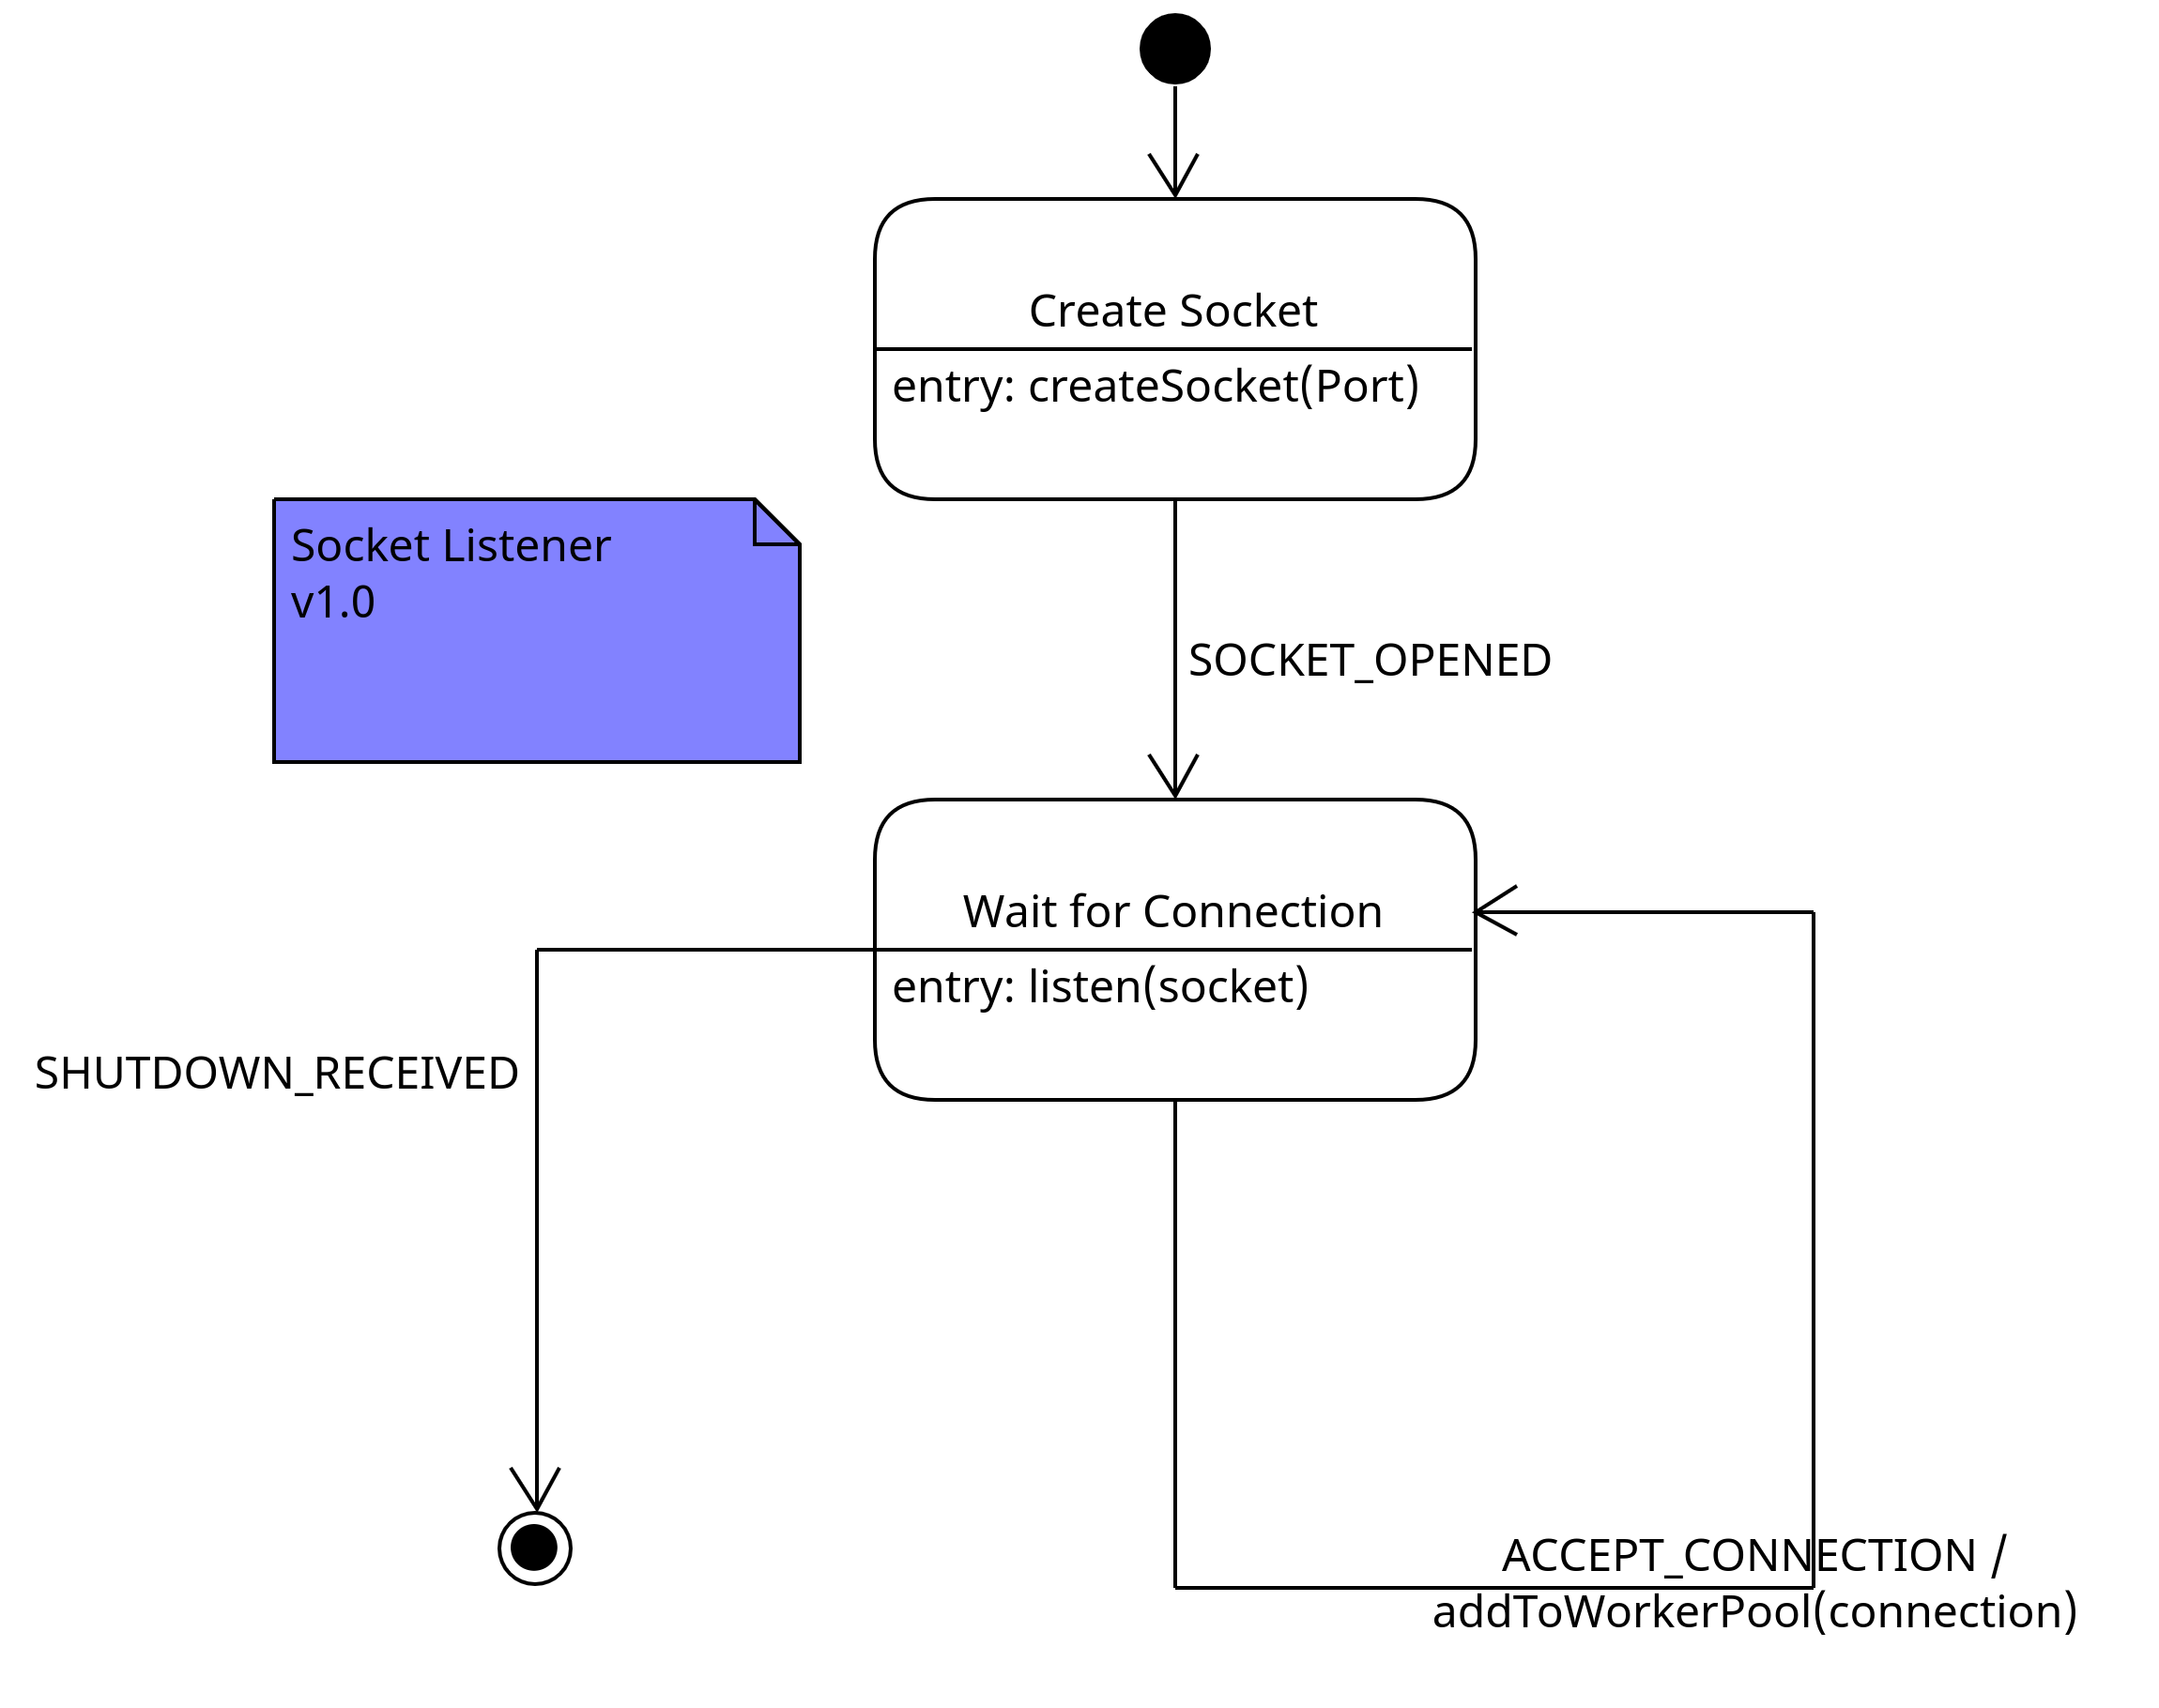
\includegraphics[width=0.8\textwidth]{images/socketlistener.png}
\caption{Socket Listener}
\label{fig:SocketListener}
\end{figure}

Um die Kommunikation mit anderen Teilnehmern des Netwerkes zu ermöglichen, wird ein Socket Listener benötigt. 
Dieser lauscht auf einem Port und empfängt Verbindungsanfragen von anderen Teilnehmern.
Diese werden dann in den Thread Pool übergeben, der die Verbindung dann in einem eigenen Thread behandelt.
Der Socket Listener wird in einem eigenen Thread ausgeführt, damit die Anwendung nicht blockiert wird.
\clearpage

\section{Tests}

\clearpage

\section{Glossar}

\begin{itemize}
    \item \textbf{Nachricht: } Eine Nachricht kann eine Chatnachricht, ein Routingpaket(siehe Chatprotokoll 3.1.2) oder ein Verbindungspaket(siehe Chatprotokoll 3.1) sein
    \item \textbf{Chatnachricht: } Eine Nachricht die einen vom Benutzer geschriebenen Text enthält und an einen anderen Benutzer addressiert ist
    \item \textbf{verfügbarer Client: } Ein Client zu dem eine direkte Verbindung besteht oder zu dem es über einen der verbundenen Clients eine Route gibt die zu dem Client führt
\end{itemize}
\clearpage

\end{document}